\documentclass[14pt]{extarticle}
% \documentclass[14pt]{article}

% \usepackage[style=authoryear,maxbibnames=9,maxcitenames=2,uniquelist=false,backend=biber,doi=false,url=false]{biblatex}
% \addbibresource{$BIB} % bibtex location
% \renewcommand*{\nameyeardelim}{\addcomma\space} % have comma in parencite
\usepackage{natbib}

\usepackage{xcolor}
\usepackage{amsmath}
\newcommand{\tuple}[1]{ \langle #1 \rangle }
%\usepackage{automata}
\usepackage{times}
\usepackage{ltablex}
\usepackage{tasks}

%%%%%% Template
\usepackage{hyperref}
\hypersetup{colorlinks=true,allcolors=blue}

\usepackage{vmargin}
\setpapersize{USletter}
\setmarginsrb{1.0in}{1.0in}{1.0in}{0.6in}{0pt}{0pt}{0pt}{0.4in}

% HOW TO USE THE ABOVE:
%\setmarginsrb{leftmargin}{topmargin}{rightmargin}{bottommargin}{headheight}{headsep}{footheight}{footskip}
%\raggedbottom
% paragraphs indent & skip:
\parindent  0.3cm
\parskip    -0.01cm

\usepackage{tikz}
\usetikzlibrary{backgrounds}

% hyphenation:
% \hyphenpenalty=10000 % no hyphen
% \exhyphenpenalty=10000 % no hyphen
\sloppy

% notes-style paragraph spacing and indentation:
\usepackage{parskip}
\setlength{\parindent}{0cm}

% let derivations break across pages
\allowdisplaybreaks

\newcommand{\orange}[1]{\textcolor{orange}{#1}}
\newcommand{\blue}[1]{\textcolor{blue}{#1}}
\newcommand{\red}[1]{\textcolor{red}{#1}}
\newcommand{\freq}[1]{{\bf \sf F}(#1)}
\newcommand{\datafreq}[2]{{{\bf \sf F}_{#1}(#2)}}

\def\qqquad{\quad\qquad}
\def\qqqquad{\qquad\qquad}

%%%%%%%%%%%%%%%%%%%%%%%%%%%%%%%%%%%%%%%%%%%%%%%%%%%%%%%%%%%%%%%%%%%%%%%%%%%%%%%%
%%%%%%%%%%%%%%%%%%%%%%%%%%%%%%%%%%%%%%%%%%%%%%%%%%%%%%%%%%%%%%%%%%%%%%%%%%%%%%%%

% fill-in-blank question style, found in https://tex.stackexchange.com/a/505089

\usepackage{ifthen}
\usepackage{tocloft}
\usepackage{exercise}
% \usepackage{xcolor}

% Set the Show Answers Boolean
\newboolean{showAns}
\setboolean{showAns}{false}
\newcommand{\showAns}{\setboolean{showAns}{true}}

% The length of the Answer line
\newlength{\answerlength}
\newcommand{\anslen}[1]{\settowidth{\answerlength}{#1}}

% ans command that indicates space for an answer or shows the answer in red
\newcommand{\ans}[1]{\settowidth{\answerlength}{\hspace{2ex}#1\hspace{2ex}}%
    \ifthenelse{\boolean{showAns}}%
        {\textcolor{red}{\underline{\hspace{2ex}#1\hspace{2ex}}}}%
        {\underline{\hspace{\answerlength}}}}%

\newcommand{\details}[1]{\settowidth{\answerlength}{#1}%
    \ifthenelse{\boolean{showAns}}%
        {\\ \textcolor{blue}{#1}}%
        {}}%

% Formatting how multiple choices Questions are formated.
\settasks{label=(\Alph*), label-width=30pt}


% Some commands for the Exercise Question package
\renewcommand{\QuestionNB}{\Large\protect\textcircled{\small\bfseries\arabic{Question}}\ }
\renewcommand{\ExerciseHeader}{} %no header
\renewcommand{\QuestionBefore}{3ex} %Space above each Q
\setlength{\QuestionIndent}{8pt} % Indent after Q number


% To create the list of answers with tocloft...
\newcommand{\listanswername}{Answers}
\newlistof[Question]{answer}{Answers}{\listanswername}

% Creates a TOC for Answers
\newcounter{prevQ}
\newcommand{\answer}[1]{\refstepcounter{answer}%
\ans{#1}%
\ifnum\theQuestion=\theprevQ%
        \addcontentsline{Answers}{answer}{\protect\numberline{}#1}% don't include the Q number
        \else%
        \addcontentsline{Answers}{answer}{\protect\numberline{\theQuestion}#1}%
        \setcounter{prevQ}{\value{Question}}%
        \fi%
        }%

% \hyphenpenalty=10000 % no hyphen
% \exhyphenpenalty=10000 % no hyphen
\sloppy              % hyphen

\newcommand{\HRule}{\rule{\linewidth}{0.5mm}}
\newcommand{\Hrule}{\rule{\linewidth}{0.3mm}}

%tocloft formatting listofanswers
\renewcommand{\cftAnswerstitlefont}{\bfseries\large}
\renewcommand{\cftanswerdotsep}{\cftnodots}
\cftpagenumbersoff{answer}
\addtolength{\cftanswernumwidth}{10pt}

\makeatletter% since there's an at-sign (@) in the command name
\renewcommand{\@maketitle}{%
  \parindent=0pt% don't indent paragraphs in the title block
  \centering
  {\Large \bfseries\textsc{\@title}} \\
  \vspace{5pt}
  {\large \textit{\@author}} \\
  \HRule \\
  \vspace{1em}
}
\makeatother% resets the meaning of the at-sign (@)


\title{ECON 2002.01 Problem Set 7 }
\author{Unit 13 \\
  \vspace{5pt}
    Hui-Jun Chen}


%%%%%%%%%%%%%%%%%%%%%%%%%%%%%%%%%%%%%%%%%%%%%%%%%%%%%%%%%%%%%%%%%%%%%%%%%%%%%%%%
%%%%%%%%%%%%%%%%%%%%%%%%%%%%%%%%%%%%%%%%%%%%%%%%%%%%%%%%%%%%%%%%%%%%%%%%%%%%%%%%
\begin{document}

\maketitle

\showAns
\listofanswer

\begin{Exercise}

\Question (OUP-U13-Q4)
The figure above shows the log of UK real GDP per capita between 1875 and 1914. Which of the following is correct?
    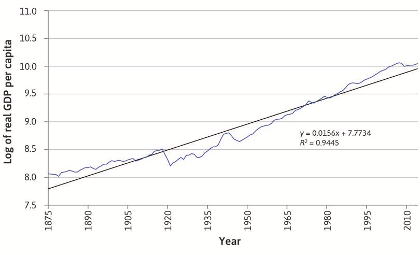
\includegraphics[width=\textwidth]{../QuestionBankImage/OUP-U13-Q04-01.png}
\answer{A}
\begin{tasks}(1)
    \task The growth of GDP in the 1950s was above the long-run average.
        \details{The slope of the blue line is steeper than that of the black line and so growth is more rapid. The fact that it lies below the black line is irrelevant.}
    \task The growth of GDP in the 1880s was above the long-run average.
        \details{The slope of the blue line is flatter than that of the black line, so the growth rate is less than the long run average. The fact that the blue line lies above the black is irrelevant.	In the figure the coefficient on x is 0.0156 and tells us the slope of the regression line (line of best fit).}
    \task If, instead, this were 0.02 the line would be flatter.
        \details{The coefficient tells us the change in the log of per capita GDP for every unit change in x where x is one year. If the coefficient were 0.2, then this would indicate that the log of per capita GDP increased each year by 2 per cent (rather than 1.56\%) and so the regression line would be steeper.}
    \task The slope of the blue line tells us the rate of growth of per capita GDP but can tell us nothing about the level.
        \details{It is correct that the slope of the blue line tells us the growth rate but each point on the blue line tells us the log of per capita GDP at that date and from the log we can calculate the actual value of GDP per capita.}
\end{tasks}



\Question (OUP-U13-Q6)
Okun's law implies that:
\answer{B}
\begin{tasks}(1)
    \task Changes in the unemployment rate and GDP growth rate are positively correlated.
        \details{This would mean that as the growth rate of output rises, unemployment also rises, which seems unlikely.}
    \task The change in unemployment is negative in booms and positive in recessions.
        \details{The data suggest that low rates of growth and employment go together. Consequently, in recessions (low growth) unemployment tends to be high. And vice versa in booms.}
    \task Every change in the level of employment is exactly matched by an opposite change in the level of unemployment.
        \details{Okun’s Law makes the point that these movements are not equal. For example, when employment rises (in a boom) unemployment will fall by a smaller number because some of the recruits will not come from the unemployed pool (new school and college leavers)}
    \task GDP growth rate and changes in unemployment are inversely correlated.
        \details{This is similar to Okun’s Law but Okun’s evidence linked unemployment to the rate of growth of GDP rather than to its level. Hence Okun was defining boom/recession as a period when growth was above/below trend, not as a period of positive or negative growth.}
\end{tasks}




\Question (OUP-U13-Q9)
The data for Spain suggests that Okun’s Law can be written as y = -0.3147x +1.2821, where y is the change in unemployment rate and x is the GDP growth rate. What is the predicted change in unemployment if GDP grows by 2 per cent?
\answer{C}
\begin{tasks}(1)
    \task Unemployment increases by 1.9115 percentage points.
        \details{1.9115 is the value we get if we ignore the negative sign on the coefficient. (1.2821 + 0.3147(2) = 1.9115).}
    \task Unemplyoment increases by 1.2758 percentage points.
        \details{1.2758 is the value we get if we enter 0.02 for 2 per cent, when the equation requires us to enter it as a whole number. (1.2821 – 0.3147(0.02) = 1.9115.}
    \task Unemployment increases by 0.6527 percentage points.
        \details{1.2821 -0.3147(2) = 0.6527}
    \task Unemployment increases by 1.2192 percentage points.
        \details{1.2192 is the value we get if we enter the growth rate as 0.2 instead of 2. 1.2821 - 0.3147(0.2) - 1.2192}
\end{tasks}



\Question (OUP-U13-Q12)
Assume that a household has access to credit. Which of the following is likely to have a significant effect on long-run consumption?
\answer{C}
\begin{tasks}(1)
    \task A temporary reduction in income.
        \details{A temporary reduction in income (a negative 'windfall') is unlikely to affect household consumption in the long-run, especially if households have access to credit. Most likely they will borrow in order to maintain their consumption plans, hoping to repay the loans when times improve.}
    \task A rise in interest rates.
        \details{The level of interest rates varies, mainly as a result of monetary policy. Changes in interest rates are therefore likely to be seen as temporary and have little effect on consumption in the long-run.}
    \task An unexpected promotion to a senior position.
        \details{A promotion to a senior position is likely mean an increase in future income over a long period. (This promotion may lead to others). If it was expected, then it might already have been taken into consumption plans and have little effect. But if it was unexpected then it is very likely to increase consumption.}
    \task A freeze in the value of state retirement benefits.
        \details{It rather depends how the freeze is interpreted. Such freezes often occur when government spending is seen to be excessive for some reason. They are essentially crisis measures and households know they will be temporary (and maybe be followed by more rapid increases later). If so, this will have little, if any, effect on long-run consumption. If, on the other hand, they were seen as part of a major ideological shift on behalf of all political parties to reduce the size of the state and to make people more responsible for their own care in old age, then the effect on consumption could be negative.}

\end{tasks}



\Question (OUP-U13-Q15)
Why is investment spending likely to be more volatile than consumption spending?
\answer{C}
\begin{tasks}(1)
    \task Because investment depends entirely on ‘animal spirits’.
        \details{It is true that he anticipated profits from investment spending depend upon a firm’s view of likely future developments and therefore upon ‘confidence’ which contains a strong psychological element. But the calculation of those likely future profits (by discounting the expected future cashflow) remains a rational exercise, albeit with some uncertainty.}
    \task Because firms cannot foresee the future.
        \details{But neither can households. Nevertheless, they try to smooth their consumption and base it upon some long-run view of what they expect to earn over a lifetime.}
    \task Because a large part of consumption spending is on items that cannot be postponed. (‘non-discretionary’) – food, heating, lighting, shelter, for example.
        \details{These items include food, heating, lighting, shelter, for example. Such spending is sometimes referred to as ‘non-discretionary’ spending.}
    \task Interest rates fluctuate.
        \details{They do, and interest rates are an important input in the investment decision. But they are relevant o consumption as well. For example, a rise in interest rates makes consuming now more ‘costly’ in relation to consuming in future because the higher interest rate generates greater income for consumption in the future period. Current consumption is likely to be reduced, rather like investment.}
\end{tasks}



\Question (OUP-U13-Q17)
Your economy is estimated to be producing about \$800bn-worth of goods and services this year. However, your official statisticians estimate that if all resources were fully-employed, it could produce about \$1000bn. The ratio 0.8 (or 80\%, $ \frac{800bn}{1000bn} $) therefore indicates:
\answer{C}
\begin{tasks}(1)
    \task The level of unemployment.
        \details{If we took the residual of 0.2 (i.e. 1 – 0.8) we would have a measure of the extent to which resources in general were underused. But ‘unemployment’ refers to the underutilisation of labour specifically. From the number 0.8 we can infer that unemployment (of labour) is likely to be positive but we cannot say more than that.}
    \task The savings ratio.
        \details{The savings ratio refers to households’ saving (non-consumption) as a fraction of their actual income. Here we have a measure of aggregate income as a fraction of potential income.}
    \task The degree of capacity utilisation.
        \details{By showing the current level of output against the maximum potential output, the degree of capacity utilisation is very useful to policymakers who may be contemplating a stimulus to the economy. It gives some indication of the size of desired stimulus.}
    \task A budget surplus.
        \details{A ‘surplus’ is involved in the sense that 0.8 shows that there is a surplus of productive capacity over what is currently being used. But the term ‘budget’ usually refers to the central government’s revenue and expenditure (and a surplus would represent an excess of revenue over expenditure). It’s also possible that a budget surplus is more likely if the economy is operating at full rather than 80\% of capacity. But the degree of capacity utilisation and a budget deficit are entirely different things’.}
\end{tasks}




\Question (OUP-U13-Q19)
In the current year, your economy is expected to make exports of \$100bn and to import \$80bn-worth of goods and services. When it comes to measuring GDP (or aggregate demand) the net effect of your external sector is to:
\answer{A}
\begin{tasks}(1)
    \task External trade contributes \$20m.
        \details{A ‘positive trade balance’ or ‘positive net exports’ are an addition to GDP (and aggregate demand). Here the contribution is \$20bn.}
    \task External trade reduces GDP by \$20bn.
        \details{A reduction in GDP (and aggregate demand) would require negative net exports, i.e. X < M. But here the difference is positive.}
    \task We cannot tell.
        \details{Most official statistics come with a margin of error. But there’s no reason to suppose that import/export figures are particularly unreliable. There is one thing that we do not know, however. Like any autonomous addition to aggregate demand, net exports are likely to have secondary, subsequent effects. They may start by boosting aggregate demand by \$20bn but that increase may lead to further increases through a process known as the multiplier. Without knowing the value of the multiplier we cannot know the ultimate effect of net exports. We look at the multiplier process in Unit 14.}
    \task It depends on the composition of imports and exports.
        \details{The initial impact on GDP depends only on the size of the expenditure. The earnings from the sale of services, for example, are just as relevant as the earnings from goods. Of course, there will be other effects which do depend on the composition. If UK cars become very fashionable with overseas buyers, the car industry will expand and the area of its location will become more prosperous. However, if foreign cars become more fashionable in the UK, the reverse will happen.}
\end{tasks}




\Question (OUP-U13-Q21)
The Consumer Price Index (CPI):
\answer{C}
\begin{tasks}(1)
    \task Records the price of all goods and services in the economy.
        \details{Not all goods and services. It records the prices of what consumers actually buy and reflects the importance (or ‘weight’) of those items in the overall household budget.}
    \task Records the price of all goods produced in the domestic economy, including exports.
        \details{It records the prices of services as well. It also excludes the prices of exports (bought by overseas consumers) but does include the prices of imports.}
    \task Measures the general level of prices that consumers pay for goods and services.
        \details{It records the prices of goods and services in a typical ‘shopping basket’. The items and their weights are based upon a continuous sampling of consumer spending habits.}
    \task Measures the rate of inflation.
        \details{No. The CPI records the general level of prices. Inflation is the rate of change of prices.}
\end{tasks}



\Question (OUP-U13-Q13)
A temporary change in income affects the current consumption of credit-constrained households more than it does that of the unconstrained because:
\answer{B}
\begin{tasks}(1)
    \task A credit-constrained household is unlikely to have savings to fall back on.
        \details{Not necessarily. Borrowing (using credit) and saving are different things. Financial institutions may be unwilling to extend credit to certain types of household but they are unlikely to decline their savings. If credit-constrained households lack savings, it must be for some additional reason.}
    \task If the household cannot borrow, its current consumption is limited by its current income.
        \details{If it cannot borrow, then it cannot consume more than its income.}
    \task A credit-constrained household cannot foresee the future.
        \details{Foreseeing the future is difficult for everyone. It is not peculiar to credit-constrained households. The problem with credit constraints is not that they prevent one from looking ahead, but that the prevent one from taking action to deal with what one foresees.}
    \task Credit-constrained households are likely to be shortsighted.
        \details{Taking only a very short-term view is likely to tie consumption more closely to income since temporary changes in income will not be seen as temporary. But there’s no reason to suppose that this is necessarily a characteristic of credit-constrained households.}
\end{tasks}

\newpage

\Question (OUP-U13-Q16)
The figure shows that total investment spending can be volatile because the interaction of individual firms’ decisions can lead to vicious (low profit) or virtuous (high profit) circles. Which of the following might encourage all firms in the economy to behave in such a way that they all increase their investment spending together?
    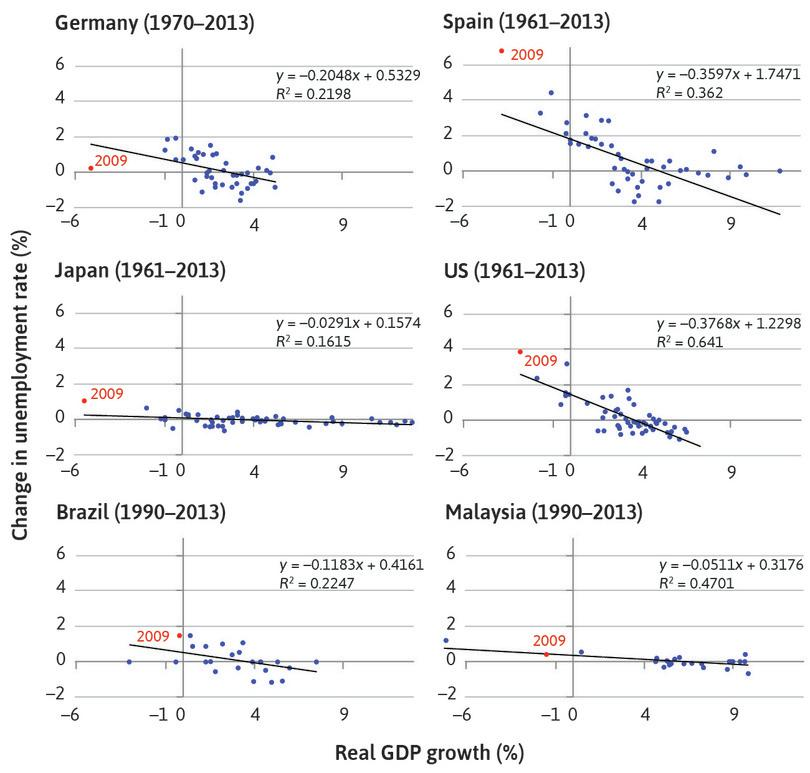
\includegraphics[width=\textwidth]{../QuestionBankImage/OUP-U13-Q7-01.jpg}

\answer{C}
\begin{tasks}(1)
    \task A fall in the exchange rate (the domestic currency becomes cheaper for foreign buyers).
        \details{This makes exports cheaper and imports dearer. Net exports are likely to increase and that will give boost to aggregate demand. But the positive effect will be limited to firms with significant exports and firms that have to buy materials from overseas will find their costs rising (and sales possibly falling).Also, fluctuations in exchange rates happen frequently. Any rise or fall is likely to be temporary. So a general boost to investment is unlikely.}
    \task A major technological breakthrough – say in batteries for electric cars.
        \details{Clearly, this is likely to encourage more investment in the automobile industry and in battery manufacture. Some firms may also recognise it as having implications for their industry even though they don’t make electric cars. But even with this ‘good news effect’ technological breakthroughs, however, general their application are unlikely to encourage all firms to expand investment simultaneously.}
    \task The use by government of fiscal policy to increase aggregate demand.
        \details{An increase in aggregate demand will encourage all firms to expect a higher demand for their products and this should have a beneficial effect on investment plans across the economy. This will be especially true if the policy is given lots of publicity and if the government’s promises are seen as credible.}
    \task Calls from government for firms to increase investment.
        \details{This is unlikely to have much effect. Firms undertake investment in order to remain competitive and/or to expand production. They do this because they see the possibility of profit and their shareholders will expect them to make the best decisions with respect to profit. Investments risky and firms are unlikely to undertake it just because governments ask them to do it. However, such encouragement might have some effect if combined with the publicity surrounding an expansionary fiscal policy.}
\end{tasks}

\end{Exercise}

\end{document}
